\section{Part I: Stochastic Gradient Descent}

Stochastic Gradient Descent~\cite{robbins1951stochastic} (SGD) is a fundamental optimisation algorithm widely used for training neural networks. Its primary goal is to minimise an objective function—in this case, the average loss over the training dataset—by iteratively updating the model’s weight parameters. Unlike traditional gradient descent, which computes the gradient using the entire dataset, SGD estimates the gradient using a small subset of the data (a mini-batch), thereby significantly reducing the computational cost per update and introducing beneficial stochasticity into the learning process.

Assume the objective function is defined as the average loss over \( n \) training samples:
\[
    f(w) = \frac{1}{n} \sum_{i=1}^{n} L_i(x_i, w)
\]
where \( L_i(x_i, w) \) is the loss for the \( i^{\text{th}} \) sample \( x_i \) with model parameters \( w \). The full gradient of this function is given by:
\[
    \nabla f(w) = \frac{1}{n} \sum_{i=1}^{n} \nabla L_i(x_i, w).
\]

To overcome the computational overhead of processing the complete dataset at each update, SGD approximates this gradient using a mini-batch of \( m \) training samples. The corresponding weight update rule is formulated as:
\[
    w = w - \eta \left( \frac{1}{m} \sum_{i=1}^{m} \nabla L_i(x_i, w) \right),
\]
where: \( \eta \) is the learning rate that governs the magnitude of the update and \( \nabla L_i(x_i, w) \) represents the gradient of the loss for the \( i^{\text{th}} \) training sample.

The main reasons for employing SGD include:
\begin{itemize}
  \item \textbf{Computational Efficiency}: By using only a fraction of the data for each update, SGD significantly reduces the amount of computation required per iteration~\cite{bottou2010large}.
  \item \textbf{Noise Regularization}: Stochastic updates use smaller learning rates to temper gradient noise, yielding smoother convergence \citep{WilsonMartinez2003}; this noise also serves as an implicit regularizer, and averaged stochastic gradients converge to the true gradient over time \citep{GoodfellowBengioCourville2016}.
  \item \textbf{Flat Minima} By using small batches, SGD avoids the sharp minima that large‑batch methods often converge to, and sharp minima that degrade model quality and impair generalization \cite{MishkinSergievskiyMatas2017, KeskarEtAl2017}.
\end{itemize}




\subsection{Stochastic Gradient Descent Implementation}

A function named \texttt{update\_parameters()}  completes the SGD implementation by updating the weight matrices using the rule:
\[
    w = w - \eta \frac{dw}{m},
\]
where \(\eta\) (the learning rate) is set to 0.1 and \(m\) (the batch size) is set to 10. The function sequentially calls \texttt{update\_weights()} for each weight matrix associated with the network layers:
\begin{itemize}
    \item \(W_{LI,L1}\) (Input to first hidden layer),
    \item \(W_{L1,L2}\) (First to second hidden layer),
    \item \(W_{L2,L3}\) (Second to third hidden layer), and
    \item \(W_{L3,LO}\) (Third hidden to output layer).
\end{itemize}
Each update subtracts the averaged gradient from the current weight, and then resets the gradient accumulator to zero, thus ensuring that the parameter updates correctly reflect the gradient descent step derived from the mini-batch.


\subsection{Validation through Numerical Differentiation}

Numerical differentiation is used to validate the analytically computed gradients. Three methods are implemented:

\begin{itemize}
    \item \textbf{Forward Difference:} Approximates the gradient by perturbing the weight positively:
    \[
        \frac{\partial f}{\partial w} \approx \frac{f(w + \epsilon) - f(w)}{\epsilon}
    \]
    \item \textbf{Backward Difference:} Approximates the gradient by perturbing the weight negatively:
    \[
        \frac{\partial f}{\partial w} \approx \frac{f(w) - f(w - \epsilon)}{\epsilon}
    \]
    \item \textbf{Central Difference:} Uses both forward and backward perturbations to obtain a more accurate estimate:
    \[
        \frac{\partial f}{\partial w} \approx \frac{f(w + \epsilon) - f(w - \epsilon)}{2\epsilon}
    \]
\end{itemize}

In these formulas, \(\epsilon\) is a small constant used to perturb the weights, with \(\epsilon = 10^{-8}\). These methods provide numerical approximations that can be compared against the analytical gradients to ensure the correctness of the backpropagation implementation.


\subsection{Results and Discussion}

\begin{figure}[ht]
    \centering
    % First sub-figure: Combined training plot (loss and accuracy over iterations)
    \begin{minipage}[t]{0.45\textwidth}
        \centering
        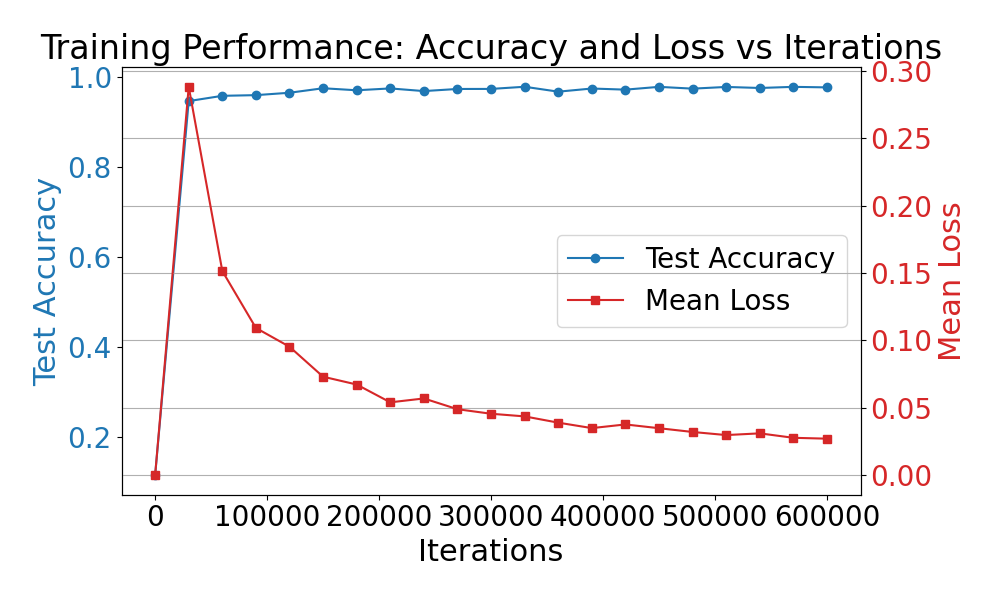
\includegraphics[width=\linewidth]{../data/part1/combined_training_plot}
        \caption{Training Performance: Loss and Accuracy over Iterations}
        \label{fig:combined_training_plot}
    \end{minipage}
    \hfill
    % Second sub-figure: Accuracy around the optima (>30000 iterations)
    \begin{minipage}[t]{0.45\textwidth}
        \centering
        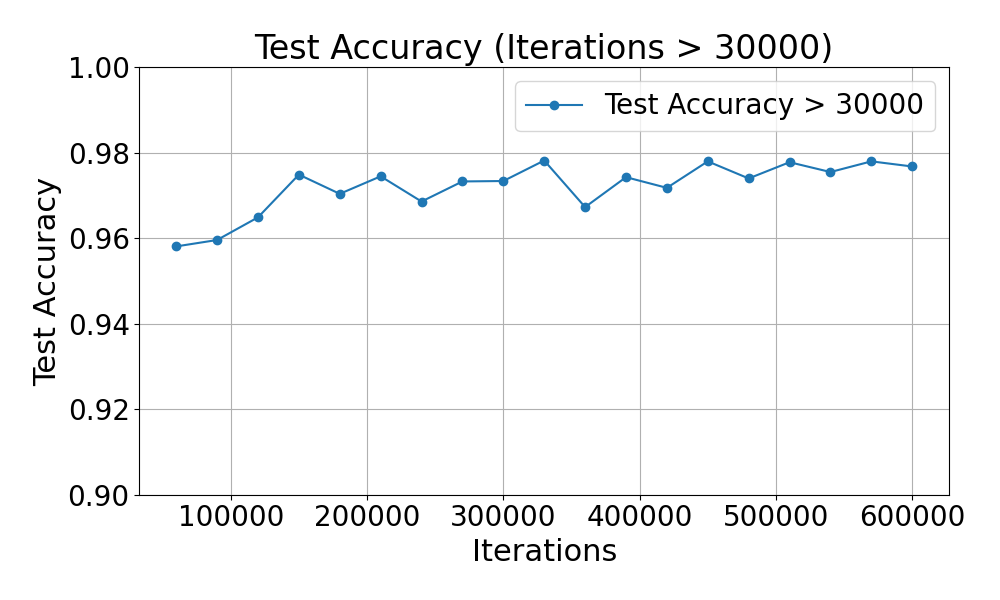
\includegraphics[width=\linewidth]{../data/part1/accuracy_after30000}
        \caption{Detailed Accuracy after 30000 Iterations}
        \label{fig:accuracy_after30000}
    \end{minipage}
    \hfill
\end{figure}

\begin{wraptable}{r}{0.38\textwidth}
    \centering
    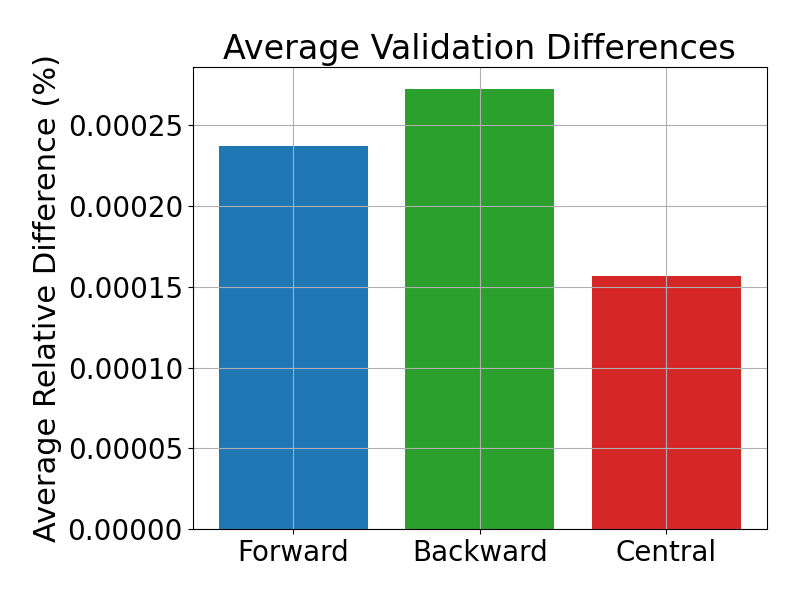
\includegraphics[width=\linewidth]{../data/part1/validation_comparison}
    \caption{Gradient Validation: Relative Difference Comparison}
    \label{fig:validation_comparison}
\end{wraptable}

Figure~\ref{fig:validation_comparison} compares the gradient validation results using forward, backward, and central differencing methods. The central difference method yields the lowest average relative difference because its symmetric formulation cancels the first-order error terms, providing a second-order accurate estimate~\cite{burden2000numerical}. In contrast, the forward and backward difference methods are only first-order accurate. This enhanced accuracy of the central difference method justifies its preference for gradient validation. Meanwhile, the average relative difference results are small enough to confirm that the analytical gradients are correct, as all methods yield values below 0.0003\%.

Regarding the compute time, the numerical methods incur significant computational cost since each estimate requires multiple function evaluations per parameter. Based on the empirical results, the forward differencing method takes approximately 0.52123 seconds per sample, the backward differencing method requires 0.52331 seconds per sample, and the central differencing method incurs a cost at 0.52957 seconds per sample. On the other hand, the analytical gradient computation, achieved through backpropagation, computes the full gradient vector in a single, efficient backward pass, making it substantially faster.

Figure~\ref{fig:combined_training_plot} reveals that, starting near 10\% at iteration 0, the test accuracy rapidly surpasses 90\% by 30{,}000 iterations, reflecting the network’s rapid acquisition of fundamental features. Beyond 30{,}000 iterations, the loss decreases from around 0.3 to below 0.05 as the optimiser fine-tunes the parameters. Figure~\ref{fig:accuracy_after30000} focuses on iterations exceeding 30{,}000, where the accuracy fluctuates between approximately 96\% and 98\%. This plateau indicates that SGD has converged to a (local) optimum.

